%%%%%%%%%%%%%%%%%%%%%%%%%%%%%%%%%%%%%%%%%%%%%%%%%%%%%%%%%%%%%
%% Begin exercise %%
%%%%%%%%%%%%%%%%%%%%%%%%%%%%%%%%%%%%%%%%%%%%%%%%%%%%%%%%%%%%%
\ex{Transistor-based AC-DC converters}

%%%%%%%%%%%%%%%%%%%%%%%%%%%%%%%%%%%%%%%%%%%%%%%%%%%%%%%%%%%%%
%% Task 1: Single-phase inverter: %%
%%%%%%%%%%%%%%%%%%%%%%%%%%%%%%%%%%%%%%%%%%%%%%%%%%%%%%%%%%%%%

\task{Single-phase AC-DC converter}
The following ideal single-phase converter
%%%%%%%%%%%%%%%%%%%%%%%%%%%%%%%%%%%%%%%%%%%%%%%%%%%%%%%%%%%%%
%% Single-phase DC inverter with inductive filter %%
%%%%%%%%%%%%%%%%%%%%%%%%%%%%%%%%%%%%%%%%%%%%%%%%%%%%%%%%%%%%%

\begin{figure}[htb]
    \begin{center}
        \begin{circuitikz}
            % Add voltage U1p
            \draw (0,0) coordinate (U1) to [open, o-o, v = $U_1\hspace{0.5cm}$, voltage = straight] ++(0,-5.5) coordinate (Gnd)
            % Add current
            (U1) to [short, o-, i=$i_1(t)$] ++(2,0) coordinate (jT1c)
            % Add T1
            (jT1c) to [Tnpn, n=T1, invert, bodydiode] ++(0,-2) coordinate (jT1e)
            % Add connection to u2
            (jT1e) to [short, *-] ++(1,0) to [crossing] ++(2,0) coordinate (ju2)
            % Add u2 inductor
            (ju2) to [L, l=$L$, name = L] ++(2,0)  to [short] ++(0.1,0) coordinate (ju2e)          
            % Add junction to T2
            (jT1e) to [short] ++(0,-1.5) coordinate (jT2c)
            % Add T2
            (jT2c) to [Tnpn, n=T2, invert, bodydiode] ++(0,-2) coordinate (jT2e)
            % Add connection to T3
            (jT1c) to [short, *-] ++(2,0) coordinate (jT3c)
            % Add T3
            (jT3c) to [Tnpn, n=T3, invert, bodydiode] ++(0,-2) coordinate (jT3e)
            % Add junction to ju2
            (jT3e) to [short] ++(0,-0.5) coordinate (jmu2)
            % Add junction to T4
            (jmu2) to [short] ++(0,-1) coordinate (jT4c)
            % Add T4
            (jT4c) to [Tnpn, n=T4, invert, bodydiode] ++(0,-2) coordinate (jT4e)
            % Add connection to T2
            (jT4e) to [short, -*] (jT2e)
            % Add connection to Gnd U1
            (jT2e) to [short, -] (Gnd)
            % Add connection to u2 inductor
            (jmu2) to [short,-] ++(0,2) coordinate (ju2x)
            % Add u2ae
            (ju2e) to [sV=$u_{2\mathrm{i}}(t)$] ++(0,-1.5) coordinate (ju2n)
            % Add connection of u2in
            (ju2n) to [short,-*] (jT4c);


            % Add component name of transistors
            \draw let \p1 = (T1.B) in node[anchor=east] at (\x1,\y1) {$T_1$};
            \draw let \p1 = (T2.B) in node[anchor=east] at (\x1,\y1) {$T_2$};
            \draw let \p1 = (T3.B) in node[anchor=east] at (\x1,\y1) {$T_3$};
            \draw let \p1 = (T4.B) in node[anchor=east] at (\x1,\y1) {$T_4$};
            % Add current arrows i2
            \draw (jT1e) ++(3,0) node[currarrow](i2){}
            (i2)  node[anchor=south,color=black]{$i_\mathrm{2}(t)$}
            % Add voltage arrows u2
            (ju2) ++(-0.5,0) to [open,v^=$$,voltage = straight] ++(0,-1.5)
            (ju2) ++ (0.1,-0.5) node[anchor=north,color=black]{$u_\mathrm{2}(t)$};
           % (ju2x) ++(0,-0.8) to [open,v^=$u_\mathrm{2}(t)$,voltage = straight] ++(3.8,0);
        \end{circuitikz}
    \end{center}
    \caption{Single-phase AC-DC converter}
    \label{fig:Fig_Single-phase_DC_Inverter}
\end{figure}

 

configured in a bridge topology and supplies a load consisting of an inductor and an internal load voltage. The converter consists
of four transistors arranged in full bridge configuration.

\begin{table}[ht]
    \centering  % Zentriert die Tabelle
    \begin{tabular}{ll}
        \toprule
        Input DC voltage: & $U_{\mathrm{1}}=\SI{200}{\volt}$ \\
        Inductance: & $L = \SI{4.8}{\milli \henry}$ \\
        Internal load voltage: & $u_{2\mathrm{i}}(t) = 150 \sin(\omega t - \frac{\pi}{6})$ \\ 
        Reference angular frequency: & $\omega_2 = 2\pi \cdot \SI{50}{\hertz}$ \\ 
        \bottomrule
    \end{tabular}
    \caption{Parameters of the single-phase AC-DC converter.}  
    \label{table:ex07_Task1_ParametersOfTheCircuit}
\end{table}
The converter is modulated using PWM with a modulation index of $m=0.75$.  Assuming ideal operation of the switching components, perform the following tasks:
% Subtask1
\subtask{Draw the converter's output voltage $u_\mathrm{2}(t)$ belonging to Fig. \ref{sfig:ex07_sub1.1_modulation}.
and its fundamental component $u^\mathrm{(1)}_\mathrm{2}(t)$. How large is the phase difference $\varphi_{2\mathrm{i}}$ of the voltage
fundamental component $u^\mathrm{(1)}_\mathrm{2}(t)$ compared to the internal load voltage $u_{2\mathrm{i}}(t)$?}

\begin{solutionblock}
    Considering the modulation in Fig. \ref{sfig:ex07_sub1.1_modulation}, the output voltage $u_\mathrm{2}(t)$ can either be $+U_1$ or $-U_1$ based on
    the maximum between the carrier signal $c(t)$ and reference $s^{*}(t)$, as shown in the figure. Moreover, the amplitude of the fundamental component $u^\mathrm{(1)}_\mathrm{2}(t)$ of the output voltage can be calculated using the modulation
    index $m$ as:
    \begin{equation}
        m = \frac{\hat{u}^\mathrm{(1)}_\mathrm{2}}{U_{\mathrm{1}}}, \hat{u}^\mathrm{(1)}_\mathrm{2} = 0.75 U_{\mathrm{1}} =  \SI{150}{\volt},
        \label{7.1.1:eq:mag_u2_fund}         
    \end{equation}

    \begin{equation}
        \varphi_{2\mathrm{i}} = \SI{\frac{\pi}{6}}{\radian}.
        \label{7.1.1:eq:varphi_2i}         
    \end{equation}
\end{solutionblock}
%\begin{figure}[htb]
%    \begin{center}
%        \begin{circuitikz}
%            \begin{scope}[yshift=-9cm, local bounding box=sawtooth]
                %\draw (0,-1) -- ++(0,2) -- ++(2,-2) -- ++(0,2) -- ++(2,-2) -- ++(0,2) -- ++(2,-2);
                % the above line does the same as the following one, but without the foreach loop
%                \draw (0,-1) foreach \x in {1,2,3} {-- ++(2,2) -- ++(0,-2) };
%            \end{scope}
%        \end{circuitikz}
%    \end{center}
%    \caption{Single-phase DC Inverter}
   % \label{fig:Fig_Single-phase_DC_Inverter}
%\end{figure}
%%%%%%%%%%%%%%%%%%%%%%%%%%%%%%%%%%%%%%%%%%%%%%%%%%%%%%%%%%%%%%%%%%%%%%%%%%
% Fundamental Current i^1_1a for M3C with RL-Load
%%%%%%%%%%%%%%%%%%%%%%%%%%%%%%%%%%%%%%%%%%%%%%%%%%%%%%%%%%%%%%%%%%%%%%%%%%
\begin{figure}[htb]

    %   \documentclass{standalone}
    %   \usepackage{pgfplots}
    %   \pgfplotsset{compat=1.18} % Kompatibilität für neuere Versionen
           \centering
           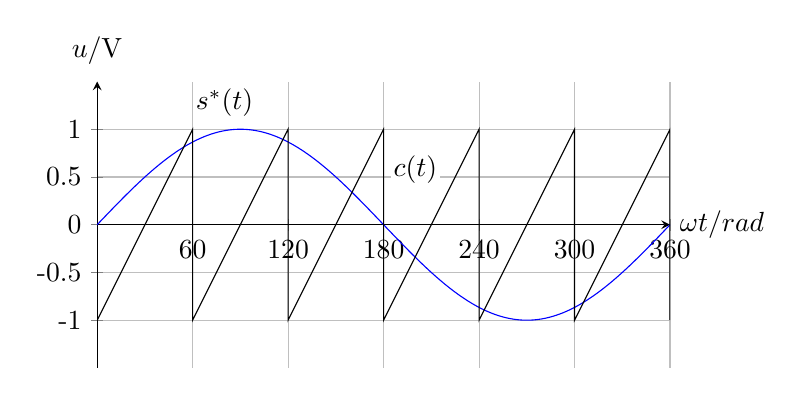
\begin{tikzpicture}
                \pgfplotsset{set layers}
           \begin{axis}[
            % x/y range adjustment
            scale only axis,
            ymin=-1.5, ymax=1.5,
            xmin=0, xmax=360, 
            samples=500,
            axis y line=center,
            axis x line=middle,
            extra y ticks=0,
            % Label text
            xlabel={$\omega t / \text{rad}$},
            ylabel={$u/\mathrm{V}$},
            % Label adjustment
            x label style={at={(axis description cs:1,0.5)},anchor=west},
            y label style={at={(axis description cs:0,.97)},anchor=south,yshift=0.2cm},
            width=0.6\textwidth,
            height=0.3\textwidth,
            % x-Ticks
            xtick={0,60,120,180,240, 300, 360},
            xticklabels={0,60,120,180,240, 300, 360},
            xticklabel style = {anchor=north},
            % y-Ticks
            ytick={-1,-0.5,0,0.5,1},
            yticklabels={-1,-0.5,0,0.5,1},
            yticklabel style = {anchor=east},
            % Grid layout
            grid,
            %grid style={line width=.1pt, draw=gray!10},
            %major grid style={line width=.2pt,draw=gray!90},
        ] 
        % modulation s
        \addplot[blue, domain= 0:360, solid] {sin(x)};
      % carrier signal c
       \draw[thin, black] (0,-1) -- (60,1) -- (60,-1) -- (120,1) -- (120,-1) -- (180,1) -- (180,-1) -- (240,1) -- (240,-1) -- (300,1) -- (300,-1) -- (360,1) -- (360,-1);
        %\draw (0,-1) \foreach \x in {0 ,60, 120, 180, 240, 300} {-- ++(60,2) -- ++(0,-2) };
        
        % Label of s
        \node[black, fill=white, inner sep = 1pt, anchor = south] at (axis cs:80,1.1) {$s^{*}(t)$};
        % Label of c
        \node[black, fill=white, inner sep = 1pt, anchor = south] at (axis cs:200,0.4) {$c(t)$};
           \end{axis}         
           \end{tikzpicture}
           \caption{Carrier signal $c(t)$ and reference $s^{*}(t)$.}
           \label{sfig:ex07_sub1.1_modulation}
   \end{figure}

% Subtask2
\subtask{Calculate the amplitude $\hat{i}^\mathrm{(1)}_\mathrm{2}$ and the phase angle $\varphi^\mathrm{(1)}$ of the 
current fundamental component $i^\mathrm{(1)}_\mathrm{2}(t)$ compared to $u_{2\mathrm{i}}(t)$, and draw $u^\mathrm{(1)}_\mathrm{2}(t)$ 
as well as $i^\mathrm{(1)}_\mathrm{2}(t)$ in Fig. \ref{sfig:ex07_sub1.2_fund_components}.}

\begin{solutionblock}
    %\input{fig/ex07/steady_state_operation_7.1.2.tex}
    Starting with the fundamental component of the output voltage $u^\mathrm{(1)}_\mathrm{2}(t)$, which can be expressed as:
    \begin{equation}
        u^\mathrm{(1)}_\mathrm{2}(t) = u_{2\mathrm{i}}(t) + u^\mathrm{(1)}_{\mathrm{L}}(t) = u_{2\mathrm{i}}(t) + \mathrm{j} \omega_\mathrm{2} L i^\mathrm{(1)}_\mathrm{2}(t).
        \label{7.1.2:eq:u_2_fund}         
    \end{equation}
   
    Solving for $i^\mathrm{(1)}_\mathrm{2}(t)$ leads to:
    \begin{equation}
        i^\mathrm{(1)}_\mathrm{2}(t) = \frac{u^\mathrm{(1)}_\mathrm{2}(t) - u_{2\mathrm{i}}(t)}{\mathrm{j} \omega_\mathrm{2} L},
        \label{7.1.2:eq:i_2_fund}         
    \end{equation}
    which can be represented in phasor as 
    \begin{equation}
        \underline{i}^\mathrm{(1)}_\mathrm{2} = \frac{\hat{u}^\mathrm{(1)}_\mathrm{2} e^{\mathrm{j} \cdot 0} - \hat{u}_{2\mathrm{i}} e^{\mathrm{j} \cdot \frac{\pi}{6}}}{\mathrm{j} \omega_\mathrm{2} L} = \frac{\hat{u}^\mathrm{(1)}_\mathrm{2} - \hat{u}_{2\mathrm{i}} \cos(\frac{\pi}{6}) + \mathrm{j} \hat{u}_{2\mathrm{i}} \sin(\frac{\pi}{6})}{\mathrm{j} \omega_\mathrm{2} L}.
        \label{7.1.2:eq:i_2_fund_phasor}         
    \end{equation}
    After simplification, the final expression for the fundamental current $\underline{i}^\mathrm{(1)}_\mathrm{2}$ is 
    \begin{equation}
        \underline{i}^\mathrm{(1)}_\mathrm{2} = \frac{\hat{u}_{2\mathrm{i}} \sin(\frac{\pi}{6})}{\mathrm{j} \omega_\mathrm{2} L} - \mathrm{j} \frac{\hat{u}^\mathrm{(1)}_\mathrm{2} - \hat{u}_{2\mathrm{i}} \cos(\frac{\pi}{6})}{\mathrm{j} \omega_\mathrm{2} L} = \hat{i}^\mathrm{(1)}_\mathrm{2} e^{\mathrm{j} \cdot \varphi_\mathrm{i}}.
        \label{7.1.2:eq:i_2_fund_simplified}         
    \end{equation}
    The magnitude $\hat{i}^\mathrm{(1)}_\mathrm{2}$ can be calculated using 
    \begin{equation}
        \hat{i}^\mathrm{(1)}_\mathrm{2} = \frac{1}{\omega_\mathrm{2} L}\sqrt{(\hat{u}_{2\mathrm{i}} \sin(\frac{\pi}{6}))^2 + (\hat{u}^\mathrm{(1)}_\mathrm{2} - \hat{u}_{2\mathrm{i}} \cos(\frac{\pi}{6}))^2} \approx \SI{51.5}{\ampere},
        \label{7.1.2:eq:mag_i_2_fund}         
    \end{equation}
    while the phase $\varphi^\mathrm{(1)}$ can be obtained from
    \begin{equation}
        \varphi^\mathrm{(1)} = \arctan(\frac{-\hat{u}^\mathrm{(1)}_\mathrm{2} + \hat{u}_{2\mathrm{i}} \cos(\frac{\pi}{6})}{\hat{u}_{2\mathrm{i}} \sin(\frac{\pi}{6})}) \approx \SI{-0.26}{\radian},
        \label{7.1.2:eq:phase_i_2_fund}         
    \end{equation}
    where 
    \begin{equation}
        \hat{u}^\mathrm{(1)}_\mathrm{2} =  \hat{u}_{2\mathrm{i}} = m U_1 = \SI{150}{\volt}. 
        \label{7.1.2:eq:u_2_fund_ui}          
    \end{equation}
    Consequently, the expressions for $u^\mathrm{(1)}_\mathrm{2}(t)$ and $i^\mathrm{(1)}_\mathrm{2}(t)$ are
    \begin{equation}
        \begin{aligned}
            &u^\mathrm{(1)}_\mathrm{2}(t) = m U_{\mathrm{1}} \sin(\omega_2 t),\\
            &i^\mathrm{(1)}_\mathrm{2}(t) = \hat{i}^\mathrm{(1)}_\mathrm{2} \sin(\omega_2 t - \varphi^\mathrm{(1)}).
        \end{aligned}
        \label{7.1.2:eq:i_u_2_fund}          
    \end{equation}
\end{solutionblock}

%%%%%%%%%%%%%%%%%%%%%%%%%%%%%%%%%%%%%%%%%%%%%%%%%%%%%%%%%%%%%%%%%%%%%%%%%%%%%%%%%%%%%
% Fundamental Current i^1_1 and fundamental volage u^1_2 for single-phase DC inverter
%%%%%%%%%%%%%%%%%%%%%%%%%%%%%%%%%%%%%%%%%%%%%%%%%%%%%%%%%%%%%%%%%%%%%%%%%%%%%%%%%%%%%
\begin{figure}[h!]

    %   \documentclass{standalone}
    %   \usepackage{pgfplots}
    %   \pgfplotsset{compat=1.18} % Kompatibilität für neuere Versionen
           \centering
           \begin{tikzpicture}
                \pgfplotsset{set layers}
           \begin{axis}[
            % x/y range adjustment
            scale only axis,
            ymin=-200, ymax=200,
            xmin=0, xmax=360, 
            samples=500,
            axis y line=center,
            axis x line=middle,
            extra y ticks=0,
            % Label text
            xlabel={$\omega t / \text{rad}$},
            ylabel={$u/\mathrm{V}$},
            % Label adjustment
            x label style={at={(axis description cs:1.05,0.5)},anchor=west},
            y label style={at={(axis description cs:0,.97)},anchor=south,yshift=0.2cm},
            width=0.6\textwidth,
            height=0.3\textwidth,
            % x-Ticks
            xtick={0,60,120,180,240, 300, 360},
            xticklabels={0,$\frac{\pi}{3}$,$\frac{2\pi}{3}$,$\pi$,$\frac{4\pi}{3}$, $\frac{5\pi}{3}$, $2\pi$},
            xticklabel style = {anchor=north},
            % y-Ticks
            ytick={-200,-100,0,100,200},
            yticklabels={-200,-100,0,100,200},
            yticklabel style = {anchor=east},
            % Grid layout
            grid,
            thick
            %grid style={line width=.1pt, draw=gray!10},
            %major grid style={line width=.2pt,draw=gray!90},
        ] 
        % internal load voltage u_2i
        \addplot[signalalpha, domain= 0:360, solid, thick] {150*sin(x-(180/6))};
        % Label of u_2i
        \node[signalalpha, fill=white, inner sep = 1pt, anchor = south] at (axis cs:120,160) {$u_{2\mathrm{i}}(t)$};
        \begin{solutionblock}
        % fundamental voltage u^(1)_2
        \addplot[signalbeta, domain= 0:360, solid, thick] {150*sin(x)};
         % Label of u^(1)_2
         \node[signalbeta, fill=white, inner sep = 1pt, anchor = south] at (axis cs:70,155) {$u^\mathrm{(1)}_\mathrm{2}(t)$};
        \end{solutionblock}
           \end{axis}
           \begin{axis}[
            % x/y range adjustment
            scale only axis,
            ymin=-100, ymax=100,
            xmin=0, xmax=360,
            axis x line=none, 
            samples=500,
            axis y line=right,
            axis x line=middle,
            extra y ticks=0,
            % Label text
            ylabel={$i/\mathrm{A}$},
            % Label adjustment
            y label style={rotate = -90,at={(axis description cs:1,.97)},anchor=south,yshift=0.2cm},
            width=0.6\textwidth,
            height=0.3\textwidth,
            % y-Ticks
            ytick={-100,-50,0,50,100},
            yticklabels={-100,-50,0,50,100},
            yticklabel style = {anchor=west},
            % Grid layout
            grid,
            thick
            %grid style={line width=.1pt, draw=gray!10},
            %major grid style={line width=.2pt,draw=gray!90},
        ]
        \begin{solutionblock}
              % fundamental current i^(1)_2
              \addplot[signaldelta, domain= 0:360, solid, thick] {51.5*sin(x-14.9)};
                % Label of i^(1)_2
                \node[signaldelta, fill=white, inner sep = 1pt, anchor = south] at (axis cs:100,25) {$i^\mathrm{(1)}_\mathrm{2}(t)$};
            \end{solutionblock}
           \end{axis}             
           \end{tikzpicture}
           \caption{Internal load voltage $u_{2\mathrm{i}}(t)$, fundamental voltage and current components $u^\mathrm{(1)}_\mathrm{2}(t)$
            and  $i^\mathrm{(1)}_\mathrm{2}(t)$, respectively. }
           \label{sfig:ex07_sub1.2_fund_components}
   \end{figure}
% Subtask3
\subtask{In Fig. \ref{sfig:ex07_sub1.3_Harmonics}, draw the voltage harmonics $u^{(\mathrm{h})}_\mathrm{2}(t)$. Try to sketch, approximately,
the current harmonics $i^{(\mathrm{h})}_\mathrm{2}(t)$ by counting the voltage time area squares. 
One square corresponds to a voltage time area of $\SI{25.9}{\milli \volt \second}$. The starting point is marked with \textbf{x}.\\

Hint:  The current harmonics $i^{(\mathrm{h})}_\mathrm{2}(t)$ are free of any bias.}
\begin{solutionblock}
    The harmonics $u^{(\mathrm{h})}_\mathrm{2}(t)$ can be calculated from the output voltage $u_\mathrm{2}(t)$ and the fundamental component $u^{(1)}_\mathrm{2}(t)$ with
    \begin{equation}
        u^{(\mathrm{h})}_\mathrm{2}(t) = u_\mathrm{2}(t) - u^{(1)}_\mathrm{2}(t),
        \label{7.1.2:eq:u_2_harm}         
    \end{equation}
    
    where $u^{(1)}_\mathrm{2}(t)$ has already been calculated using \eqref{7.1.1:eq:mag_u2_fund} as
    \begin{equation}
        u^{(1)}_\mathrm{2}(t) = m U_{\mathrm{1}} \sin(\omega_2 t).         
    \end{equation}
    Hence,
    \begin{equation}
        u^{(\mathrm{h})}_\mathrm{2}(t) =  \begin{cases}
            - m U_{\mathrm{1}} \sin(\omega_2 t) + U_{\mathrm{1}} &\text{ when $T_1$ and $T_4$ are conducting,}\\
            - m U_{\mathrm{1}} \sin(\omega_2 t)  - U_{\mathrm{1}} &\text{ when $T_2$ and $T_3$ are conducting}.
            \end{cases}
        \label{7.1.2:eq:u_2_harm_cases}         
    \end{equation}
    Consequently, the change in the harmonics of the output current $\Delta i^{(\mathrm{h})}_\mathrm{2}$ between $t_0$ and $t_1$ can be expressed as 
    \begin{equation}
        \Delta i^{(\mathrm{h})}_\mathrm{2} = \frac{1}{L} \int_{t_0}^{t_1} u^{(\mathrm{h})}_\mathrm{2}(t) \mathrm{d}t = \frac{1}{L} \int_{t_0}^{t_1} u_\mathrm{2}(t) - u^{(1)}_\mathrm{2}(t) \mathrm{d}t.
        \label{7.1.2:eq:i_2_harm}         
    \end{equation}
    For hand sketching, a simple graphical solution can be obtained by counting the number of squares below $u^{(\mathrm{h})}_\mathrm{2}(t)$, hence,
    each step $\Delta i^{(\mathrm{h})}_\mathrm{2}$ can be approximated with:
        \begin{equation}
            \Delta i^{(\mathrm{h})}_\mathrm{2} = \frac{1}{L} \cdot \text{(number of squares)} \cdot \SI{25.9}{\milli \volt \second}.
            \label{7.1.2:eq:approx_i_2_harm}         
        \end{equation}
        For example, the change in the current staring from \textbf{x} until the time of the first switching $t_1$ from $U_1$ to $-U_1$ can be calculated as:
        \begin{equation}
            \Delta i^{(\mathrm{h})}_\mathrm{2} = \frac{1}{\SI{4.8}{\milli \henry}} \cdot 14 \cdot \SI{25.9}{\milli \volt \second} \approx \SI{75.5}{\ampere},
            \label{7.1.2:eq:approx_i_2_harm_example}         
        \end{equation}
        where $14$ is, approximately, the number of squares below $u^{(\mathrm{h})}_\mathrm{2}(t)$ in this time interval. So, the current at the first switching time $t_1$ is:
        \begin{equation}
            i^{(\mathrm{h})}_\mathrm{2}(t_1) = i^{(\mathrm{h})}_\mathrm{2}(t_0) + \Delta i^{(\mathrm{h})}_\mathrm{2} = -44.4 + 75.5 \approx \SI{31}{\ampere}.
            \label{7.1.2:eq:approx_i_2_harm_t1}         
        \end{equation}
        The next steps $\Delta i^{(\mathrm{h})}_\mathrm{2}$ in the trajectory of $i^{(\mathrm{h})}_\mathrm{2}(t)$ can be calculated in the same way
        using the corresponding 'number of squares'.  
\end{solutionblock}
%%%%%%%%%%%%%%%%%%%%%%%%%%%%%%%%%%%%%%%%%%%%%%%%%%%%%%%%%%%%%%%%%%%%%%%%%%%%%%%%%%%%%
% Fundamental Current i^1_1 and fundamental volage u^1_2 for single-phase DC inverter
%%%%%%%%%%%%%%%%%%%%%%%%%%%%%%%%%%%%%%%%%%%%%%%%%%%%%%%%%%%%%%%%%%%%%%%%%%%%%%%%%%%%%
\begin{figure}[h!]

    %   \documentclass{standalone}
    %   \usepackage{pgfplots}
    %   \pgfplotsset{compat=1.18} % Kompatibilität für neuere Versionen
           \centering
           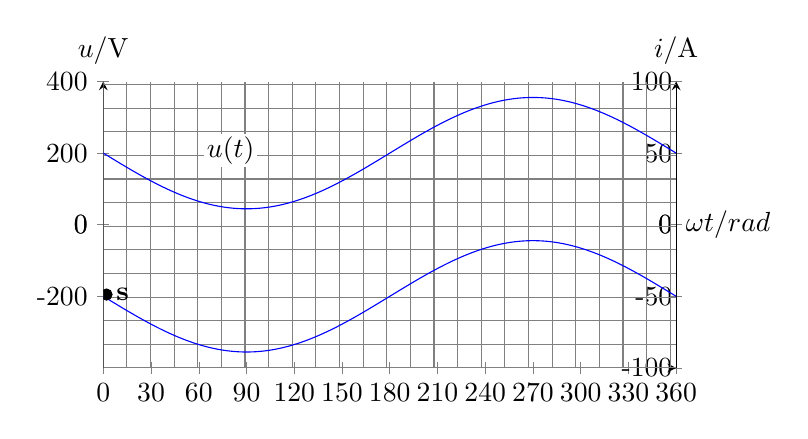
\begin{tikzpicture}
                \pgfplotsset{set layers}
           \begin{axis}[
            % x/y range adjustment
            scale only axis,
            ymin=-400, ymax=400,
            xmin=0, xmax=540, 
            samples=500,
            axis y line=center,
            axis x line=bottom,
            extra y ticks=0,
            % Label text
            xlabel={$\omega t / \text{rad}$},
            ylabel={$u/\mathrm{V}$},
            % Label adjustment
            x label style={at={(axis description cs:1,0.5)},anchor=west},
            y label style={at={(axis description cs:0,.97)},anchor=south,yshift=0.2cm},
            width=0.6\textwidth,
            height=0.3\textwidth,
            % x-Ticks
            xtick={0, 45, 90, 135, 180, 225, 270, 315, 360, 405, 450,495, 540},
            xticklabels={0, 30, 60, 90, 120, 150, 180, 210, 240, 270, 300, 330, 360},
            xticklabel style = {anchor=north},
            % y-Ticks
            ytick={-400,-200,0,200,400},
            yticklabels={-400,-200,0,200,400},
            yticklabel style = {anchor=east},
            % Grid layout
           % grid,
            %grid style={line width=.1pt, draw=gray!10},
            %major grid style={line width=.2pt,draw=gray!90},
        ] 
        % Grid
        \draw[step=0.3cm, gray, thin] (0,-400) grid (540,400);
        % internal load voltage u
        \addplot[blue, domain= 0:540, solid] {-155.5*sin(x/1.5)+200};
        \addplot[blue, domain= 0:540, solid] {-155.5*sin(x/1.5)-200};
         % Label of u
         \node[black, fill=white, inner sep = 1pt, anchor = south] at (axis cs:120,160) {$u(t)$};
         % Start point
         \filldraw[black] (3,-195) circle (2pt) node[anchor=west]{\textbf{s}};
           \end{axis}
           \begin{axis}[
            % x/y range adjustment
            scale only axis,
            ymin=-100, ymax=100,
            xmin=0, xmax=360,
            axis x line=none, 
            samples=500,
            axis y line=right,
            axis x line=middle,
            extra y ticks=0,
            % Label text
            ylabel={$i/\mathrm{A}$},
            % Label adjustment
            y label style={rotate = -90,at={(axis description cs:1,.97)},anchor=south,yshift=0.2cm},
            width=0.6\textwidth,
            height=0.3\textwidth,
            % y-Ticks
            ytick={-100,-50,0,50,100},
            yticklabels={-100,-50,0,50,100},
            yticklabel style = {anchor=east},
            % Grid layout
           % grid,
            %grid style={line width=.1pt, draw=gray!10},
            %major grid style={line width=.2pt,draw=gray!90},
        ]
           \end{axis}             
           \end{tikzpicture}
           \caption{Harmonics of the output voltage and current.}
           \label{sfig:ex07_sub1.3_Harmonics}
   \end{figure}
\newpage
% Subtask4
\subtask{Draw the converter's output current $i_\mathrm{2}(t)$, its fundamental component $i^\mathrm{(1)}_\mathrm{2}(t)$ 
and its harmonics $i^{(\mathrm{h})}_\mathrm{2}(t)$ in Fig. \ref{sfig:ex07_sub1.4_current_and_components}.}
\begin{solutionblock}
The fundamental component $i^\mathrm{(1)}_\mathrm{2}(t)$ and the harmonics $i^{(\mathrm{h})}_\mathrm{2}(t)$ have already been calculated in subtasks 7.1.2 and 7.1.3. Hence,
the output current $i_\mathrm{2}(t)$ of the converter can be calculated using 
\begin{equation}
    i_\mathrm{2}(t) = i^\mathrm{(1)}_\mathrm{2}(t) + i^{(\mathrm{h})}_\mathrm{2}(t).
    \label{7.1.2:eq:approx_i_2}         
\end{equation}
\end{solutionblock} 
%%%%%%%%%%%%%%%%%%%%%%%%%%%%%%%%%%%%%%%%%%%%%%%%%%%%%%%%%%%%%%%%%%%%%%%%%%%%%%%%%%%%%
% Fundamental Current i^1_1 and fundamental volage u^1_2 for single-phase DC inverter
%%%%%%%%%%%%%%%%%%%%%%%%%%%%%%%%%%%%%%%%%%%%%%%%%%%%%%%%%%%%%%%%%%%%%%%%%%%%%%%%%%%%%
\begin{figure}[h]

    %   \documentclass{standalone}
    %   \usepackage{pgfplots}
    %   \pgfplotsset{compat=1.18} % Kompatibilität für neuere Versionen
           \centering
           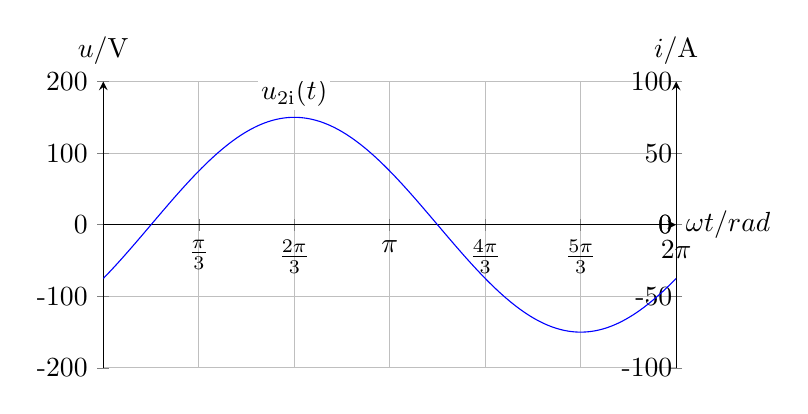
\begin{tikzpicture}
                \pgfplotsset{set layers}
           \begin{axis}[
            % x/y range adjustment
            scale only axis,
            ymin=-200, ymax=200,
            xmin=0, xmax=360, 
            samples=500,
            axis y line=center,
            axis x line=middle,
            extra y ticks=0,
            % Label text
            xlabel={$\omega t / \text{rad}$},
            ylabel={$u/\mathrm{V}$},
            % Label adjustment
            x label style={at={(axis description cs:1,0.5)},anchor=west},
            y label style={at={(axis description cs:0,.97)},anchor=south,yshift=0.2cm},
            width=0.6\textwidth,
            height=0.3\textwidth,
            % x-Ticks
            xtick={0,60,120,180,240, 300, 360},
            xticklabels={0,$\frac{\pi}{3}$,$\frac{2\pi}{3}$,$\pi$,$\frac{4\pi}{3}$, $\frac{5\pi}{3}$, $2\pi$},
            xticklabel style = {anchor=north},
            % y-Ticks
            ytick={-200,-100,0,100,200},
            yticklabels={-200,-100,0,100,200},
            yticklabel style = {anchor=east},
            % Grid layout
            grid,
            %grid style={line width=.1pt, draw=gray!10},
            %major grid style={line width=.2pt,draw=gray!90},
        ] 
        % internal load voltage u
        \addplot[blue, domain= 0:360, solid] {150*sin(x-(180/6))};
         % Label of u
         \node[black, fill=white, inner sep = 1pt, anchor = south] at (axis cs:120,160) {$u_{2\mathrm{i}}(t)$};
           \end{axis}
           \begin{axis}[
            % x/y range adjustment
            scale only axis,
            ymin=-100, ymax=100,
            xmin=0, xmax=360,
            axis x line=none, 
            samples=500,
            axis y line=right,
            axis x line=middle,
            extra y ticks=0,
            % Label text
            ylabel={$i/\mathrm{A}$},
            % Label adjustment
            y label style={rotate = -90,at={(axis description cs:1,.97)},anchor=south,yshift=0.2cm},
            width=0.6\textwidth,
            height=0.3\textwidth,
            % y-Ticks
            ytick={-100,-50,0,50,100},
            yticklabels={-100,-50,0,50,100},
            yticklabel style = {anchor=east},
            % Grid layout
            grid,
            %grid style={line width=.1pt, draw=gray!10},
            %major grid style={line width=.2pt,draw=gray!90},
        ]
           \end{axis}             
           \end{tikzpicture}
           \caption{Output current $i_\mathrm{2}(t)$, its fundamental wave $i^\mathrm{(1)}_\mathrm{2}(t)$ 
           and its harmonics $i^{(k)}_\mathrm{2}(t)$. }
           \label{sfig:ex07_sub1.4_current_and_components}
   \end{figure}

% Subtask5
\subtask{Mark the input current $i_\mathrm{1}(t)$ of the AC-DC converter in Fig. \ref{sfig:ex07_sub1.4_current_and_components}.}
\begin{solutionblock}
    The input current $i_\mathrm{1}(t)$ can be calculated from $i_\mathrm{2}(t)$ using 
    \begin{equation}
        i_\mathrm{1}(t) = s(t) i_\mathrm{2}(t),
        \label{7.1.2:eq:input_current_i_1}         
    \end{equation}
    where $s(t)$ is the switching function. Fig. \ref{sfig:ex07_sub1.4_current_and_components} shows the input current's trajectory
    compared to the output current $i_\mathrm{2}(t)$.
    \end{solutionblock}








\newpage
%%%%%%%%%%%%%%%%%%%%%%%%%%%%%%%%%%%%%%%%%%%%%%%%%%%%%%%%%%%%%
%% Task 2: Three-phase inverter in six-step mode         %%
%%%%%%%%%%%%%%%%%%%%%%%%%%%%%%%%%%%%%%%%%%%%%%%%%%%%%%%%%%%%%

\task{Symmetrical 3-phase rectifier}

A rectifier in three-phase bridge topology shall supply a
symmetrical three-phase load in star connection. The load is represented by an inductance and 
a sinusoidal internal (or inner) voltage per phase. The inverter is operated with the fundamental 
frequency modulation (also known as six-step mode) and the switching elements are considered as ideal. 
The schematic is depicted in \autoref{fig:Fig_ThreePhaseInverter_6StepMode}.

%%%%%%%%%%%%%%%%%%%%%%%%%%%%%%%%%%%%%%%%%%%%%%%%%%%%%%%%%%%%%%%%%%%%%%%
 % Fig_ThreePhaseInverter_6StepMode
%%%%%%%%%%%%%%%%%%%%%%%%%%%%%%%%%%%%%%%%%%%%%%%%%%%%%%%%%%%%%%%%%%%%%%%
    \begin{figure}[htb]
        \begin{center}
            \begin{circuitikz}
                % Add voltage U1p
                \draw (0,0) coordinate (U1p) to [open, o-o, v = $\frac{U_1}{2}\hspace{0.5cm}$, voltage = straight] ++(0,-2.5) coordinate (Gnd)
                (Gnd) node[rground, rotate = 270 ](){} ++(0.4,0)
                (Gnd) to [open, -o, v = $\frac{U_1}{2}\hspace{0.5cm}$, voltage = straight] ++(0,-2.5) coordinate (U1m)
                % Add current
                (U1p) to [short, o-, i=$i_1(t)$] ++(2,0) coordinate (jT1c)
                % Add T1
                (jT1c) to [Tnpn, n=T1, invert, bodydiode] ++(0,-2) coordinate (jT1e)
                % Add connection to u2a
                (jT1e) to [short, *-] ++(1,0) to [crossing] ++(2,0) to [crossing] ++(2,0) to [short,-] ++(3,0) coordinate (ju2a)          
                % Add junction to T2
                (jT1e) to [short] ++(0,-1) coordinate (jT2c)
                % Add T2
                (jT2c) to [Tnpn, n=T2, invert, bodydiode] ++(0,-2) coordinate (jT2e)
                % Add connection to T3
                (jT1c) to [short, *-] ++(2,0) coordinate (jT3c)
                % Add T3
                (jT3c) to [Tnpn, n=T3, invert, bodydiode] ++(0,-2) coordinate (jT3e)
                % Add junction to ju2b
                (jT3e) to [short] ++(0,-0.5) coordinate (jmu2b)
                % Add connection to u1b
                (jmu2b) to [short,*-] ++(1,0) to [crossing] ++(2,0) to [short,-] ++(3,0) coordinate (ju2b)
                % Add junction to T4
                (jmu2b) to [short] ++(0,-0.5) coordinate (jT4c)
                % Add T4
                (jT4c) to [Tnpn, n=T4, invert, bodydiode] ++(0,-2) coordinate (jT4e)
                % Add connection to T5
                (jT3c) to [short, *-] ++(2,0) coordinate (jT5c)
                % Add T5
                (jT5c) to [Tnpn, n=T5, invert, bodydiode] ++(0,-2) coordinate (jT5e)
                % Add junction to T6
                (jT5e) to [short] ++(0,-1) coordinate (jT6c)
                % Add T6
                (jT6c) to [Tnpn, n=T6, invert, bodydiode] ++(0,-2) coordinate (jT6e)
                % Add connection to T4
                (jT6e) to [short, -*] (jT4e)
                % Add connection to T2
                (jT4e) to [short, -*] (jT2e)
                % Add connection to U1m
                (jT2e) to [short, -] (U1m)
                % Add 2. Ground symbol
                (jmu2b) ++(4.7,-2.6) node[rground](){} coordinate (Gnd2)
                % Add connection to u2c
                (jT6c) to [short,*-] ++(4,0) coordinate (ju2c)
                % Add connection to u2a inductor
                (ju2a) to [short,-] ++(0,2) coordinate (ju2ax)
                % Add u2a inductor
                (ju2ax) to [L, l=$L$, name = L] ++(2,0) coordinate (ju2ae)
                % Add u2ae
                 (ju2ae) to [sV=$u_\mathrm{2ai}$] ++(1.5,0) coordinate (ju2an)
                % Add u2b inductor
                (ju2b) to [L, l=$L$, name = L] ++(2,0) coordinate (ju2be)
                % Add u2be
                 (ju2be) to [sV=$u_\mathrm{2bi}$] ++(1.5,0) coordinate (ju2bn)
                % Add connection to u2c inductor
                (ju2c) to [short,-] ++(0,-2) coordinate (ju2cx)
                % Add u2a inductor
                (ju2cx) to [L, l=$L$, name = L] ++(2,0) coordinate (ju2ce)
                % Add u2ce
                (ju2ce) to [sV=$u_\mathrm{2ci}$] ++(1.5,0) coordinate (ju2cn)
                % Add connection of u2in
                (ju2an) to [short,-*] (ju2bn) to [short,-] (ju2cn)
                % Add connection point u2n
                (ju2bn) to [short,-o] ++(0.6,0) coordinate (ju2n)
                % Add 3. Ground symbol
                (ju2n) ++(0,-2.6) node[rground](){} coordinate (Gnd3);


                % Add component name of transistors
                \draw let \p1 = (T1.B) in node[anchor=east] at (\x1,\y1) {$T_1$};
                \draw let \p1 = (T2.B) in node[anchor=east] at (\x1,\y1) {$T_2$};
                \draw let \p1 = (T3.B) in node[anchor=east] at (\x1,\y1) {$T_3$};
                \draw let \p1 = (T4.B) in node[anchor=east] at (\x1,\y1) {$T_4$};
                \draw let \p1 = (T5.B) in node[anchor=east] at (\x1,\y1) {$T_5$};
                \draw let \p1 = (T6.B) in node[anchor=east] at (\x1,\y1) {$T_6$};
                % Add current arrows i2a, i2b and i2c
                \draw (jT1e) ++(1,0) node[currarrow](i2a){}
                (i2a)  node[anchor=north,color=black]{$i_\mathrm{2a}(t)$}
                (jmu2b) ++(1,0) node[currarrow](i2b){}
                (i2b)  node[anchor=north,color=black]{$i_\mathrm{2b}(t)$}
                (jT6c) ++(1,0) node[currarrow](i2c){}
                (i2c)  node[anchor=north,color=black]{$i_\mathrm{2c}(t)$}
                % Add voltage arrow u1
                (U1p) ++(0.3,0.5) to [open,v^=$$,voltage = straight] ++(0,-6)coordinate (Uges)
                (Uges) ++ (0.3,3) node[anchor=north,color=black]{$U_\mathrm{1}$}
                % Add voltage arrow u2an, u2bn and u2cn
                (ju2ax) ++(0,-0.8) to [open,v^=$u_\mathrm{2a}(t)$, voltage = straight] ++(3.8,0)
                (ju2b) ++(0,-0.8) to [open,v^=$u_\mathrm{2b}(t)$,voltage = straight] ++(3.8,0)
                (ju2cx) ++(0,-0.8) to [open,v^=$u_\mathrm{2c}(t)$,voltage = straight] ++(3.8,0)
                % Add voltage arrow u2ab
                (ju2ax) ++(0.2,0) to [open,v^=$$,voltage = straight] ++(0,-2.5)
                (ju2ax) ++ (0.9,-1) node[anchor=north,color=black]{$u_\mathrm{2ab}(t)$}
                % Add voltage arrow u2bc
                (ju2b) ++(0.2,0) to [open,v^=$$,voltage = straight] ++(0,-2.5)
                (ju2b) ++ (0.9,-1) node[anchor=north,color=black]{$u_\mathrm{2bc}(t)$}
                % Add voltage arrow ua0
                (Gnd2) ++(-0.7,3.4) to [open,v^=$$,voltage = straight] ++(0,-3.6)
                (Gnd2) ++ (-1.4,1.2) node[anchor=north,color=black,rotate = 90]{$u_\mathrm{2a0}(t)$}
                % Add voltage arrow ub0
                (Gnd2) ++(0,2.9) to [open,v^=$$,voltage = straight] ++(0,-3.01)
                (Gnd2) ++ (-0.7,1.2) node[anchor=north,color=black,rotate = 90]{$u_\mathrm{2b0}(t)$}
                % Add voltage arrow uc0
                (Gnd2) ++(0.7,2.4) to [open,v^=$$,voltage = straight] ++(0,-2.42)
                (Gnd2) ++ (0,1.2) node[anchor=north,color=black,rotate = 90]{$u_\mathrm{2b0}(t)$}
                % Add voltage arrow un0
                (Gnd3) ++(0,2.8) to [open,v^=$$,voltage = straight] ++(0,-3.01)
                (Gnd3) ++ (-0.7,1.2) node[anchor=north,color=black,rotate = 90]{$u_\mathrm{2n0}(t)$};



            \end{circuitikz}
        \end{center}
        \caption{Three-phase inverter in six-step mode.}
        \label{fig:Fig_ThreePhaseInverter_6StepMode}
    \end{figure}




\begin{table}[ht]
    \centering  % Center the table
    \begin{tabular}{ll}
        \toprule
        Input voltages: & $U_\mathrm{1}=\SI{510}{\volt}$ \\
        Internal voltages: & $u_{\mathrm{2ai}}(t) = \sqrt{2} \cdot \SI{220}{\volt} \cdot \sin(\omega_1t)$ \\
        Angular load frequency: & $\omega_1 = \SI{2 \pi \cdot 30}{\frac{1}{\second}}$ \\ 11
        Inductance per phase: & $L= \SI{10}{\milli \henry}$ \\
        Phase angle between  $u_{\mathrm{2ai}}(t)$ and $i_{\mathrm{2ai}}^\mathrm{(1)}(t)$ & $\varphi_{\mathrm{2a}}^\mathrm{(1)}=\SI{30}{\degree}$ \\
        \bottomrule
    \end{tabular}
    \caption{Parameters of three-phase inverter in six-step mode.}  
    \label{table:ex07_Task2_ParametersOfTheCircuit}
\end{table}

\subtask{Create a table with all possible switching states for fundamental frequency modulation.
Use the following notation:
\begin{align*}
    \{ s_\mathrm{a}(t),s_\mathrm{b}(t),s_\mathrm{c}(t) \}=\begin{cases}
        s_i(t)= +1 & \text{upper position,}\\
        s_i(t)= -1 & \text{lower position.}
    \end{cases}
\bigskip    
\end{align*}
Sketch the switching states in the correct chronological order for one period.
Calculate and sketch the voltages $u_\mathrm{2a0}(t)$, $u_\mathrm{2b0}(t)$ and $u_\mathrm{2c0}(t)$ 
depending on these switching states.}
\begin{solutionblock}
    Each half bridge has got the 2 states '+1' and '-1', which results in $2^3 = 8$ combinations according table \autoref{stable:ex07_Task2_Switchingstates}.
    To simplify the entries following is defined: $U_\mathrm{1h}=\frac{U_\mathrm{1}}{2}.$
    The correct chronological order is displayed in table \autoref{stable:ex07_Task2_UsedSwitchingStates}.
    \bigskip
    \FloatBarrier

    \begin{minipage}{0.3\textwidth}
            \begin{tabular}{|c|c|c|} % Each column is separated by a line
            \hline
            \bfseries $s_\mathrm{a}(t)$ & \bfseries $s_\mathrm{b}(t)$ & \bfseries $s_\mathrm{c}(t)$ \\ \hline
            -1 & -1 & -1 \\ \hline
            -1 & -1 & +1 \\ \hline
            -1 & +1 & -1 \\ \hline
            -1 & +1 & +1 \\ \hline
            +1 & -1 & -1 \\ \hline
            +1 & -1 & +1 \\ \hline
            +1 & +1 & -1 \\ \hline
            +1 & +1 & +1 \\ \hline
        \end{tabular}
        \noindent
        \captionof{table}{Possible switching states.}
        \label{stable:ex07_Task2_Switchingstates}    
    \end{minipage}
    \hfill
    \begin{minipage}{0.55\textwidth} 
        \begin{tabular}{|c|c|c|c|c|c|} % Each column is separated by a line
            \hline
            \bfseries $s_\mathrm{a}(t)$ & \bfseries $s_\mathrm{b}(t)$ & \bfseries $s_\mathrm{c}(t)$
            & \bfseries $u_\mathrm{2a0}$ & \bfseries $u_\mathrm{2b0}$ & \bfseries $u_\mathrm{2c0}$ \\ \hline
            +1 & -1 & +1 & $U_\mathrm{1h}$ & $-U_\mathrm{1h}$ & $U_\mathrm{1h}$ \\ \hline
            +1 & -1 & -1 & $U_\mathrm{1h}$ & $-U_\mathrm{1h}$ & $-U_\mathrm{1h}$ \\ \hline
            +1 & +1 & -1 & $U_\mathrm{1h}$ & $U_\mathrm{1h}$ & $-U_\mathrm{1h}$ \\ \hline
            -1 & +1 & -1 & $-U_\mathrm{1h}$ & $U_\mathrm{1h}$ & $-U_\mathrm{1h}$ \\ \hline
            -1 & +1 & +1 & $-U_\mathrm{1h}$ & $U_\mathrm{1h}$ & $U_\mathrm{1h}$ \\ \hline
            -1 & -1 & +1 & $-U_\mathrm{1h}$ & $-U_\mathrm{1h}$ & $U_\mathrm{1h}$ \\ \hline
        \end{tabular}
        \captionof{table}{Used switching states and voltages.}
        \label{stable:ex07_Task2_UsedSwitchingStates}    
    \end{minipage}
    \bigskip
    \FloatBarrier
    The switching state (-1,-1,-1) and (+1,+1,+1) are not used. In this case the chained voltages are zero. 
    This additional degree of freedom is applied at a higher switching frequency in order to reduce the amplitude of the
    output voltage on average. In case of block switching, these switching states are not used, since
    the switching only occurs twice per period. This results in the maximum possible voltage (square wave) at the output.
    The voltages $u_\mathrm{2a0}(\mathrm{\omega t})$, $u_\mathrm{2b0}(\mathrm{\omega t})$, $u_\mathrm{2c0}(\mathrm{\omega t})$ ,$u_\mathrm{2ab}(\mathrm{\omega t})$ and $u_\mathrm{2bc}(\mathrm{\omega t})$ are displayed in \autoref{sfig:voltage_u2a0_u2b0_u2c0}.

    %%%%%%%%%%%%%%%%%%%%%%%%%%%%%%%%%%%%%%%%%%%%%%%%%%%%%%%%%%%%%%%%%%%%%%%%%%
% Voltage U_2a0 Section 
%%%%%%%%%%%%%%%%%%%%%%%%%%%%%%%%%%%%%%%%%%%%%%%%%%%%%%%%%%%%%%%%%%%%%%%%%%

\begin{solutionfigure}[ht]
    \centering
    \begin{tikzpicture}
      % groupplot begin
      \begin{groupplot}[group style={
            group size=1 by 5,
            xlabels at=edge bottom,
            y descriptions at=edge left,
          },
          width=16cm, height=10cm,
          axis lines=middle, 
          enlargelimits,
          axis line style={->}, % Pfeilspitzen an den Achsen
          xmin=0, xmax=6.2,
          ymin=-1, ymax=1,
          extra x ticks=0,
          xtick={ 1, 2, 3, 4, 5, 6},
          xticklabels={$\frac{1\pi}{3}$, $\frac{2\pi}{3}$,$\pi$, $\frac{4\pi}{3}$, $\frac{5\pi}{3}$, $2\pi$},,
          xticklabel style = {anchor=north,shift={(0.25cm,0.1cm)}},
        %  grid=both,
        ]

        \nextgroupplot[
            ymin=-1.2, ymax=1.2,
            samples=500,
            ytick distance=2,
            x label style={at={(axis description cs:1,0)},anchor=north},
            y label style={at={(axis description cs:0,.97)},anchor=south},
            height=0.2\textwidth,
            xlabel={$\omega t$},             
            ylabel={$u_\mathrm{2a0}(\omega t)/ \SI{}{\volt}$},             
            ytick={-1,0,1},
            yticklabels={$-255$,$0$,$255$},
          ]
          \addplot[color=blue,mark=none,solid] 
            coordinates{
              (0, 0)
              (0, 1)
              (3, 1)
              (3, -1)
              (6, -1)
              (6, 1)
              (6.2, 1)
          };  
          
        \nextgroupplot[
          ymin=-1.2, ymax=1.2,
          samples=500,
          ytick distance=2,
          x label style={at={(axis description cs:1,0)},anchor=north},
          y label style={at={(axis description cs:-0,.97)},anchor=south},
          height=0.2\textwidth,
          xlabel={$\omega t$},             
          ylabel={$u_\mathrm{2b0}(\omega t)/ \SI{}{\volt}$},             
          ytick={-1, 0,1},
          yticklabels={$-255$,, $255$},
        ]
        \addplot[color=blue,mark=none,solid] 
          coordinates{
            (0, -1)
            (2, -1)
            (2, 1)
            (5, 1)
            (5, -1)
            (6.2, -1)
        };  

        \nextgroupplot[
          ymin=-1.2, ymax=1.2,
          samples=500,
          ytick distance=2,
          x label style={at={(axis description cs:1,0)},anchor=north},
          y label style={at={(axis description cs:0,.97)},anchor=south},
          height=0.2\textwidth,
          xlabel={$\omega t$},             
          ylabel={$u_\mathrm{2c0}(\omega t)/ \SI{}{\volt}$},             
          ytick={-1, 0,1},
          yticklabels={$-255$,, $255$},
        ]
        \addplot[color=blue,mark=none,solid] 
          coordinates{
            (0, 1)
            (1, 1)
            (1, -1)
            (4, -1)
            (4,  1)
            (6.2,1)
        };  
    
      \end{groupplot}
    \end{tikzpicture}
    \caption{Voltage signals of $u_\mathrm{2a0}(\mathrm{\omega t})$, $u_\mathrm{2b0}(\mathrm{\omega t})$ and $u_\mathrm{2c0}(\mathrm{\omega t})$.}
    \label{sfig:voltage_u2a0_u2b0_u2c0}
\end{solutionfigure}

\end{solutionblock}

\subtask{The internal voltages $u_\mathrm{2ai}(t)$, $u_\mathrm{2bi}(t)$ and $u_\mathrm{2ci}(t)$ are from a symmetrical voltage system, 
i.e., the following is always applicable: $u_\mathrm{2ai}(t)+u_\mathrm{2bi}(t)+u_\mathrm{2ci}(t)=\SI{0}{\volt}$. 
Show that this equation is also applicable for the voltages $u_\mathrm{2a}(t)$, $u_\mathrm{2b}(t)$ and $u_\mathrm{2c}(t)$ under the same conditions.
}
\begin{solutionblock}
    In the case of a symmetrical three-phase load where the current sum at the load star point is zero, 
    the following results:
    \begin{equation}
        u_{\mathrm{2a}}(t) + u_{\mathrm{2b}}(t) + u_{\mathrm{2c}}(t) = \SI{0}{\volt} \quad 
        i_{\mathrm{2a}}(t) + i_{\mathrm{2b}}(t) + i_{\mathrm{2c}}(t) = \SI{0}{\ampere}.
        \label{eq:u2_i2_symgen}        
    \end{equation}
    This leads to
    \begin{equation}
        u_{\mathrm{2a}}(t) = L \frac{\mathrm{d}i_{\mathrm{2b}}(t)}{\mathrm{d}t}+u_{\mathrm{2ai}}(t)
        \quad u_{\mathrm{2b}}(t) = L \frac{\mathrm{d}i_{\mathrm{2b}}(t)}{\mathrm{d}t}+u_{\mathrm{2bi}}(t)
        \quad u_{\mathrm{2c}}(t) = L \frac{\mathrm{d}i_{\mathrm{2c}}(t)}{\mathrm{d}t}+u_{\mathrm{2ci}}(t).
        \label{eq:u2_i2_symL}         
    \end{equation}
    Using \eqref{eq:u2_i2_symgen} leads to
    \begin{equation}
        u_{\mathrm{2a}}(t) + u_{\mathrm{2b}}(t) + u_{\mathrm{2c}}(t) 
        = L \frac{\mathrm{d}}{\mathrm{d}t} \left( i_{\mathrm{2a}}(t)+i_{\mathrm{2b}}(t)+i_{\mathrm{2c}}(t) \right) 
         + \left( u_{\mathrm{2ai}}(t) + u_{\mathrm{2bi}}(t) + u_{\mathrm{2ci}}(t)\right)=\SI{0}{\volt}.
        \label{eq:u2_i2_symres} 
    \end{equation}
    This derivation is valid under following conditions:
    \begin{itemize}
        \item The induction $L$ is constant.
        \item The internal voltages $u_{\mathrm{2ai}}(t)$, $u_{\mathrm{2bi}}(t)$ and $u_{\mathrm{2ci}}(t)$ 
        are purely sinusoidal (no harmonics), symmetrical (sum equals zero) and independent of the currents
        $i_{\mathrm{2a}}(t)$, $i_{\mathrm{2b}}(t)$ and $i_{\mathrm{2c}}(t)$.
    \end{itemize}     
\end{solutionblock}

\subtask{Calculate and sketch the voltages $u_\mathrm{2ab}(t)$, $u_\mathrm{2bc}(t)$, $u_\mathrm{2a}(t)$ and 
the star-to-ground voltage $u_\mathrm{2n0}(t)$ depending on the switching states.}
\begin{solutionblock}
    The voltage $u_{\mathrm{2ab}}(t)$ is calculated by 
    \begin{equation}
        u_{\mathrm{2ab}}(t) =  u_{\mathrm{2a0}}(t) - u_{\mathrm{2b0}}(t).
        \label{eq:u2ab_gen}        
    \end{equation}    
    In similar way the voltage $u_{\mathrm{2bc}}(t)$ is calculated by
    \begin{equation}
        u_{\mathrm{2bc}}(t) =  u_{\mathrm{2b0}}(t) - u_{\mathrm{2c0}}(t).
        \label{eq:u2bc_gen}        
    \end{equation}    
    The voltage $u_{\mathrm{2a}}(t)$ is obtained by
    \begin{equation}
        u_{\mathrm{2a}}(t) =  u_{\mathrm{2ab}}(t) + u_{\mathrm{2b}}(t).
        \label{eq:u2a_1}        
    \end{equation}    
    Additional voltage $u_{\mathrm{2a}}(t)$ is obtained by
    \begin{equation}
        u_{\mathrm{2a}}(t) =  u_{\mathrm{2ab}}(t) +  u_{\mathrm{2bc}}(t) + u_{\mathrm{2c}}(t).
        \label{eq:u2a_2}        
    \end{equation}    
    The addition of \eqref{eq:u2a_1} and \eqref{eq:u2a_2} results in
    \begin{equation}
        2u_{\mathrm{2a}}(t) =  2u_{\mathrm{2ab}}(t) +  u_{\mathrm{2bc}}(t) 
                               + \left( u_{\mathrm{2a}}(t) + u_{\mathrm{2b}}(t) + u_{\mathrm{2c}}(t)\right)
                               - u_{\mathrm{2a}}(t).
        \label{eq:u2a_gen}        
    \end{equation}    
    Solving \eqref{eq:u2a_gen} with respect to $u_{\mathrm{2a}}(t)$ leads to
    \begin{equation}
        u_{\mathrm{2a}}(t) = \frac{2}{3} u_{\mathrm{2ab}}(t) + \frac{1}{3} u_{\mathrm{2bc}}(t).
    \end{equation}    
    The voltage $u_{\mathrm{0,n}}(t)$ is obtained by    
    \begin{equation}
        u_{\mathrm{0,n}}(t) = u_{\mathrm{2a0}}(t) - u_{\mathrm{2a}}(t)
        = u_{\mathrm{2a0}}(t) - \frac{2}{3} u_{\mathrm{2ab}}(t) - \frac{1}{3} u_{\mathrm{2bc}}(t).
    \end{equation}
    Using \eqref{eq:u2ab_gen} and \eqref{eq:u2bc_gen} leads to
    \begin{equation}
        \begin{split}
        u_{\mathrm{0,n}}(t) &= u_{\mathrm{2a0}}(t) - \frac{2}{3} \left( u_{\mathrm{2a0}}(t) - u_{\mathrm{2b0}}(t) \right) 
        - \frac{1}{3} \left( u_{\mathrm{2b0}}(t) - u_{\mathrm{2c0}}(t) \right) \\
        u_{\mathrm{0,n}}(t) &= \frac{1}{3} \left( u_{\mathrm{2a0}}(t) + u_{\mathrm{2b0}}(t) + u_{\mathrm{2c0}}(t) \right).
        \end{split}
    \end{equation}

    The voltages $u_\mathrm{2ab}(\mathrm{\omega t})$, $u_\mathrm{2bc}(\mathrm{\omega t})$, $u_\mathrm{2a}(\mathrm{\omega t})$ and $u_\mathrm{2n0}(\mathrm{\omega t})$ are depicted in \autoref{sfig:voltage_u2ab_u2bc_u2a_u2n0}.

    %%%%%%%%%%%%%%%%%%%%%%%%%%%%%%%%%%%%%%%%%%%%%%%%%%%%%%%%%%%%%%%%%%%%%%%%%%
% Voltage U_2a0 Section 
%%%%%%%%%%%%%%%%%%%%%%%%%%%%%%%%%%%%%%%%%%%%%%%%%%%%%%%%%%%%%%%%%%%%%%%%%%

\begin{solutionfigure}[ht]
    \centering
    \begin{tikzpicture}
      % groupplot begin
      \begin{groupplot}[group style={
            group size=1 by 7,
            xlabels at=edge bottom,
            y descriptions at=edge left,
          },
          width=16cm, height=10cm,
          axis lines=middle, 
          enlargelimits,
          axis line style={->}, % Pfeilspitzen an den Achsen
          xmin=0, xmax=6.2,
          ymin=-1, ymax=1,
          extra x ticks=0,
          xtick={ 1, 2, 3, 4, 5, 6},
          xticklabels={$\frac{1\pi}{3}$, $\frac{2\pi}{3}$,$\pi$, $\frac{4\pi}{3}$, $\frac{5\pi}{3}$, $2\pi$},,
          xticklabel style = {anchor=north,shift={(0.25cm,0.1cm)}},
        %  grid=both,
        ]
     
        \nextgroupplot[
          ymin=-1.2, ymax=1.2,
          samples=500,
          ytick distance=2,
          x label style={at={(axis description cs:1,0)},anchor=north},
          y label style={at={(axis description cs:0,.97)},anchor=south},
          height=0.2\textwidth,
          xlabel={$\omega t$},             
          ylabel={$u_\mathrm{2ab}(\omega t)/ \SI{}{\volt}$},             
          ytick={-1, 0,1},
          yticklabels={$-510$,, $510$},
        ]
        \addplot[color=signalalpha,mark=none,solid, thick] 
          coordinates{
            (0, 1)
            (2, 1)
            (2, 0)
            (3, 0)
            (3, -1)
            (5, -1)
            (5, 0)
            (6, 0)
            (6, 1)
            (6.2,1)
        };          

        \nextgroupplot[
          ymin=-1.2, ymax=1.2,
          samples=500,
          ytick distance=2,
          x label style={at={(axis description cs:1,0)},anchor=north},
          y label style={at={(axis description cs:0,.97)},anchor=south},
          height=0.2\textwidth,
          xlabel={$\omega t$},             
          ylabel={$u_\mathrm{2bc}(\omega t)/ \SI{}{\volt}$},             
          ytick={-1, 0,1},
          yticklabels={$-510$,,$510$},
        ]
        \addplot[color=signalalpha,mark=none,solid, thick] 
          coordinates{
            (0, -1)
            (1, -1)
            (1, 0)
            (2, 0)
            (2, 1)
            (4, 1)
            (4, 0)
            (5, 0)
            (5, -1)
            (6.2,-1)
        };                  

        \nextgroupplot[
          ymin=-430, ymax=430,
          samples=500,
          ytick distance=2,
          x label style={at={(axis description cs:1,0)},anchor=north},
          y label style={at={(axis description cs:0,.97)},anchor=south},
          height=0.2\textwidth,
          xlabel={$\omega t$},             
          ylabel={$u_\mathrm{2a}(\omega t)/ \SI{}{\volt}$},             
          ytick={-400,-200,0,200,400},
          yticklabels={$-400$, $-200$,,$200$, $400$},
        ]
        \addplot[color=signalalpha,mark=none,solid, thick] 
          coordinates{
            (0, -170)
            (0,  170)
            (1,  170)
            (1,  340)
            (2,  340)
            (2,  170)
            (3,  170)
            (3, -170)
            (4, -170)
            (4, -340)
            (5, -340)
            (5, -170)
            (6, -170)
            (6,  170)
            (6.2,170)
        };          

        \nextgroupplot[
          ymin=-120, ymax=120,
          samples=500,
          ytick distance=2,
          x label style={at={(axis description cs:1,0)},anchor=north},
          y label style={at={(axis description cs:0,.97)},anchor=south},
          height=0.2\textwidth,
          xlabel={$\omega t$},             
          ylabel={$u_\mathrm{n0}(\omega t)/ \SI{}{\volt}$},             
          ytick={-100,50,0,50,100},
          yticklabels={$-100$,,,,$100$},
        ]
        \addplot[color=signalalpha,mark=none,solid, thick] 
          coordinates{
            (0, -85)
            (0, 85)
            (1, 85)
            (1, -85)
            (2, -85)
            (2,  85)
            (3,  85)
            (3, -85)
            (4, -85)
            (4,  85)
            (5,  85)
            (5, -85)
            (6, -85)
            (6,  85)
            (6.2,85)
        };          




      \end{groupplot}
    \end{tikzpicture}
    \caption{Voltage signals of $u_\mathrm{2a}(\mathrm{\omega t})$, $u_\mathrm{2n0}(\mathrm{\omega t})$, $u_\mathrm{2ab}(\mathrm{\omega t})$ 
             and $u_\mathrm{2bc}(\mathrm{\omega t})$.}
    \label{sfig:voltage_u2ab_u2bc_u2a_u2n0}
\end{solutionfigure}


\end{solutionblock}

\subtask{Decompose the voltage $u_\mathrm{2a}(t)$ into a Fourier series and sketch the spectral lines related to the
amplitude of the fundamental signal up to order $k=13$. \\
Hint:
\begin{align*}
    b_k = \frac{4}{\pi} \int_{0}^{\frac{\pi}{2}} f(x)\sin(kx) \mathrm{d}x \quad k =\mathrm{odd}.
\end{align*}
\label{sub:DecomposeVoltage}
The formula above applies to the Fourier coefficients of an odd and alternating function.
}
\begin{solutionblock}
    In the case of odd and alternating functions corresponding to $f(x)=-f(x+\pi)$ the Fourier coefficients are:
    \begin{equation}
        \begin{split}
        a_\mathrm{k} &= 0 \\
        b_\mathrm{k} &= \frac{4}{\pi} \int_0^{\pi/2} f(x)\sin(x) \mathrm{d}x \quad k=\mathrm{odd} \\
        f(x) &= \sum_{k}^{} \left( b_k \sin(kx) \right).
       \end{split}
    \end{equation}
    The coefficients $b_k$ are the amplitudes of the respective harmonic. The voltage $u_{\mathrm{2a}}(t)$ needs 
    only to be integrated up to $\pi/2$. Only the terms with odd order numbers are taken into account.
    Apply this to the current signal is expressed by 
    \begin{equation}
        b_\mathrm{k} = \frac{4}{\pi} \int_0^{\pi/3} \frac{U_{\mathrm{1}}}{3} \sin(kt) \mathrm{d}t 
                        + \frac{4}{\pi} \int_{\pi/3}^{\pi/2} \frac{2U_{\mathrm{1}}}{3} \sin(kt) \mathrm{d}t.
    \end{equation}
    Signal ratio $u_{\mathrm{2a0}}(\omega t)/U_{\mathrm{1}}$ is depicted in \autoref{sfig:voltage_u2a0_section} for one period.
    %%%%%%%%%%%%%%%%%%%%%%%%%%%%%%%%%%%%%%%%%%%%%%%%%%%%%%%%%%%%%%%%%%%%%%%%%%
% Voltage U_um Section 
%%%%%%%%%%%%%%%%%%%%%%%%%%%%%%%%%%%%%%%%%%%%%%%%%%%%%%%%%%%%%%%%%%%%%%%%%%

\begin{solutionfigure}[ht]
    \centering
    \begin{tikzpicture}
        \begin{axis}[
          %  width=7cm, height=5cm,
            axis lines=middle, 
            enlargelimits,
            axis line style={->}, % Pfeilspitzen an den Achsen
            xlabel={$\omega t$}, 
            ylabel={$u_\mathrm{2a0}(\omega t)/ \SI{}{\volt}$}, 
            xmin=0, xmax=13/6*pi,
            ymin=-1, ymax=1,
            xtick={0,  pi/3, 2*pi/3, pi, 4*pi/3, 5*pi/3, 2*pi},
            xticklabels={0, $\frac{1\pi}{3}$, $\frac{2\pi}{3}$,$\pi$, $\frac{4\pi}{3}$, $\frac{5\pi}{3}$, $2\pi$},
            ytick={-2/3, -1/3, 0, 1/3, 2/3},
            yticklabels={$-340$, $-170$, $0$, $170$, $340$},
          %  grid=both,
          %  major grid style={line width=.2pt,draw=gray!50},
          %  minor grid style={line width=.1pt,draw=gray!20},
        ]
                \addplot[
            thick,
            mark=none,
            color=signalalpha,
            thick,
        ] coordinates {
          (0,1/3)  (1/3*pi, 1/3) (1/3*pi, 2/3)( 2/3*pi, 2/3) (2/3*pi, 1/3) (pi, 1/3) (pi, -1/3) (4/3*pi, -1/3) (4/3*pi, -1/3) (4/3*pi, -2/3) (5/3*pi, -2/3) (5/3*pi, -1/3) (2*pi, -1/3)  (2*pi, 1/3) (13/6*pi, 1/3)
        };
        \end{axis}
    \end{tikzpicture}
    \caption{Section of the voltage curve $u_\mathrm{2a0}(\mathrm{\omega t})$.}
    \label{sfig:voltage_u2a0_section}
\end{solutionfigure}
   
    \begin{equation}
        \begin{split}
            b_\mathrm{k} &= \frac{4U_{\mathrm{1}}}{3k\pi} \big[-\cos(kt)\mathrm{d}t \big]_0^{\pi/3}
            + \frac{4U_{\mathrm{1}}}{3k\pi} \big[-2\cos(kt)\mathrm{d}t \big]_{\pi/3}^{\pi/2} \\
            &= \frac{4U_{\mathrm{1}}}{3k\pi} \left(-\cos(k\frac{\pi}{3})+\cos(0) -2 \cos(k\frac{\pi}{2})+ 2\cos(0) \right) \\
            &= \frac{4U_{\mathrm{1}}}{3k\pi} \left( \cos(k\frac{\pi}{3})+ 1 -2 \cos(k\frac{\pi}{2})\right) \\
            \text{with } &\cos(k\frac{\pi}{3})+1=1.5 \quad  \text{for } k=n \cdot 6\pm1 \text{ is odd} \\
            \text{and  }&\cos(k\frac{\pi}{2})=0 \quad \text{ for } k=\text{ odd}.
        \end{split}            
    \end{equation}
    The result is displayed in the complex plane in \autoref{sfig:GraphicalSolutionOfInComplexPlane}. 

    %%%%%%%%%%%%%%%%%%%%%%%%%%%%%%%%%%%%%%%%%%%%%%%%%%%%%%%%%%%%%%%%%%%%%%%%%%
% SwitchOnBehaviorAndSwitchOffBehaviorOfUI
%%%%%%%%%%%%%%%%%%%%%%%%%%%%%%%%%%%%%%%%%%%%%%%%%%%%%%%%%%%%%%%%%%%%%%%%%%

\begin{solutionfigure}[htb]
    \centering
    \begin{minipage}[t]{0.45\textwidth}
        \centering
        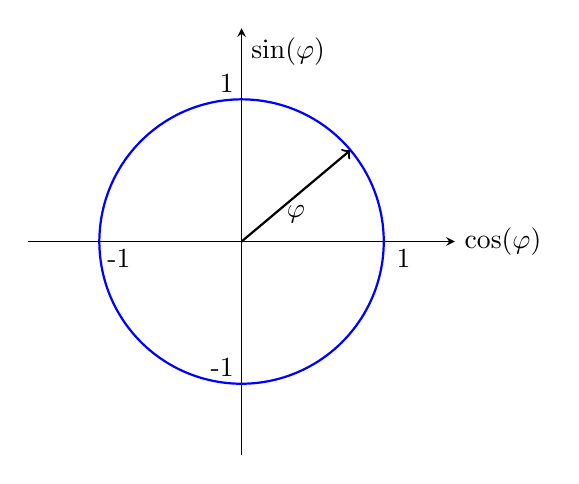
\begin{tikzpicture}
            \begin{axis}[
                % x/y range adjustment
                xmin=-20, xmax=420,
                ymin=-160, ymax=180,
                width=7cm, height=7cm,
                axis lines=middle, 
                xlabel={$\cos(\varphi)$},
                ylabel={$\sin(\varphi)$},
                major grid style={line width=.2pt,draw=gray!50},
                minor grid style={line width=.1pt,draw=gray!20},
                xmin=-1.5, xmax=1.5,
                ymin=-1.5, ymax=1.5,
                % Label adjustment
                x label style={at={(axis description cs:1,0.5)},anchor=west},
                % x-Ticks
                xtick={-1,0,1},
                xticklabels={-1,,1},
                xticklabel style = {anchor=north,shift={(0.25cm,0.1cm)}},
                % y-Ticks
                ytick={-1,0,1},
                yticklabels={-1,,1},
                yticklabel style = {anchor=east,shift={(0.1cm,0.2cm)}},
              ]
              
              \draw[thick, ->] (0,0) -- ({cos(40)}, {sin(40)}) node[above right] {};
              \node at ({0.5*cos(40)}, {0.5*sin(40)}) [below] {$\varphi$};

              \addplot[
                  domain=0:360, 
                  samples=200,  
                  thick,
                  color=blue,
              ]
              ({cos(x)}, {sin(x)}); 
            \end{axis}
        \end{tikzpicture}
    \end{minipage}
    \hspace{0.5cm}
    \begin{minipage}[t]{0.45\textwidth}
        \centering
        \begin{tikzpicture}
            \draw[->] (-2,0) -- (2,0) node[right] {}; 
            \draw[->] (0,-2) -- (0,2) node[above] {}; 
            \node at (-1.5,1.5) {$\cos\left(k \frac{\pi}{2}\right)$};
            \node at (-2,0) [left] {$k=2,6,\ldots$}; 
            \node at (2,0) [right] {$k=0,4,\ldots$}; 
            \node at (0,2) [above] {$k=1,5,9,13,\ldots$}; 
            \node at (0,-2) [below] {$k=3,7,11,15,\ldots$}; 

            % Kreuz bei jedem markierten Punkt
            \foreach \x/\y in {-1.5/0, 1.5/0, 0/1.5, 0/-1.5} {
                \draw[thick]
                    (\x,\y) +(-0.1,0.1) -- +(0.1,-0.1) % Diagonale des Kreuzes
                             +(-0.1,-0.1) -- +(0.1,0.1); % Andere Diagonale des Kreuzes
            }
        \end{tikzpicture}
    \end{minipage}
        
    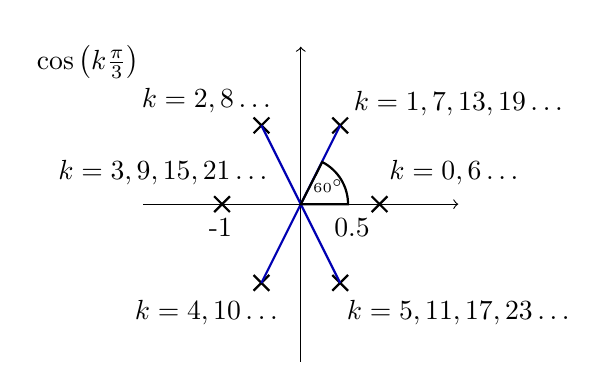
\begin{tikzpicture}
        \draw[->] (-2,0) -- (2,0) node[right] {}; 
        \draw[->] (0,-2) -- (0,2) node[above] {}; 
        \node at (-2.7,1.8) {$\cos\left(k \frac{\pi}{3}\right)$};
        \node at (-0.3,0.4) [left] {$k=3,9,15,21\ldots$}; 
        \node at (1,0.4) [right] {$k=0,6\ldots$}; 
        \node at (2,1) [above] {$k=1,7,13,19\ldots$}; 
        \node at (-1.2,1.6) [below] {$k=2,8\ldots$};
        \node at (-1.2,-1.1) [below] {$k=4,10\ldots$}; 
        \node at (2,-1.1) [below] {$k=5,11,17,23\ldots$};
        \node at (-0.75,-0.3) [left] {-1};
        \node at (1,-0.3) [left] {0.5};
        % Kreuz bei jedem markierten Punkt
        \foreach \x/\y in {-1/0, 1/0, 0.5/1, -0.5/-1, 0.5/-1, -0.5/1} {
            \draw[thick]
                (\x,\y) +(-0.1,0.1) -- +(0.1,-0.1) % Diagonale des Kreuzes
                         +(-0.1,-0.1) -- +(0.1,0.1); % Andere Diagonale des Kreuzes
        }
        \draw[thick, color=blue!70!black]
        (-0.5,1) -- (0.5,-1) -- cycle;
        \draw[thick, color=blue!70!black]
        (0.5,1) -- (-0.5,-1) -- cycle;
        \node[shift={(0.1,0)}, anchor=west] at ({0.5*cos(60)}, {0.5*sin(60)}) [below] {\tiny $60^\circ$};
        \def\drawArc#1#2#3{
        \draw[thick] (#1:0) -- (#1:#3) arc (#1:#2:#3) -- cycle;
    }
        % Beispiel: Kreissegment von 0 bis 60 Grad mit Radius 0.6
    \drawArc{0}{63}{0.6}{thick, color=blue!70!black};

    \end{tikzpicture}
    \hspace{2.3cm} % Abstand zwischen den beiden Diagrammen
    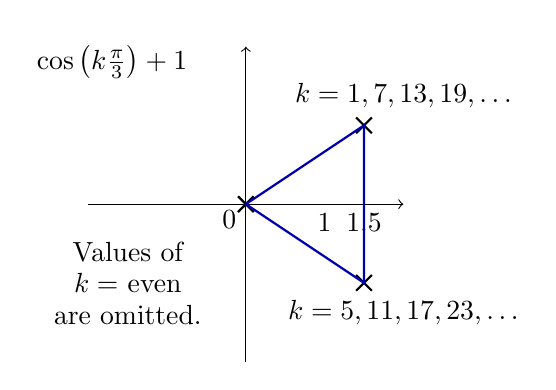
\begin{tikzpicture}
        % Koordinatensystem zeichnen
        \draw[->] (-2,0) -- (2,0) node[right] {}; 
        \draw[->] (0,-2) -- (0,2) node[above] {}; 
        % \node at (-1.5,1.5) {$\cos\left(k \frac{\pi}{3}\right)+1$};
        \node at (-1.7,1.8) {$\cos\left(k \frac{\pi}{3}\right)+1$};
        % Bemerkung
        \node at (-1.5, -0.6) {Values of};
        \node at (-1.5, -1.0) {$k=$ even};
        \node at (-1.5, -1.4) {are omitted.};
    
        % Beschriftungen an der x-Achse
        \node at (-0.00009,-0.2) [left] {0};
        \foreach \x in { 1, 1.5} {
            \node at (\x, 0) [below] {\x};
        }
    
        % Beschriftungen an spezifischen Punkten
        \node at (2,1.1) [above] {$k=1,7,13,19,\ldots$}; 
        \node at (2,-1.1) [below] {$k=5,11,17,23,\ldots$}; 
        
        
        % Kreuz bei jedem markierten Punkt
        \foreach \x/\y in {0/0, 1.5/1, 1.5/-1} {
            \draw[thick]
                (\x,\y) +(-0.1,0.1) -- +(0.1,-0.1) % Diagonale des Kreuzes
                         +(-0.1,-0.1) -- +(0.1,0.1); % Andere Diagonale des Kreuzes
        }
    
        % Verbindungslinien zwischen den Punkten
        \draw[thick, color=blue!70!black]
            (0,0) -- (1.5,1) -- (1.5,-1) -- cycle;
    \end{tikzpicture}
    \caption{Graphical solution of the cos terms within complex plane.}
    \label{sfig:GraphicalSolutionOfInComplexPlane}
\end{solutionfigure}


    \autoref{sfig:voltage_u2a0_section} leads to
    \begin{equation}
        \hat{u}_\mathrm{2a0,k} = b_\mathrm{k} = \frac{4U_{\mathrm{1}}}{3k\pi} \cdot \frac{3}{2}=\frac{2U_{\mathrm{1}}}{k\pi}.
        \label{eq:Ex07T2_FundamentelVoltage}
    \end{equation}   
    The amplitudes are depicted in \autoref{sfig:NormalizationToTheAmplitude}.
    \begin{solutionfigure}[htb]
\centering
\begin{tikzpicture}
    % Achsen zeichnen
    \draw[->] (0,0) -- (14,0) node[right] {$k$}; % x-Achse
    \draw[->] (0,0) -- (0,5) node[above] {$\frac{\hat{u}_\mathrm{2a}^\mathrm{(k)}}{\hat{u}_\mathrm{2a}^\mathrm{(1)}}$}; % y-Achse

    % Ticks und Beschriftungen auf der x-Achse
    \foreach \x in {1, 5, 7, 11, 13} {
        \draw (\x,0.05) -- (\x,-0.05) node[below] {\x};
    }
    \foreach \x in {2, 3, 4, 6, 8, 9, 10, 12} {
        \draw (\x,0.02) -- (\x,-0.02); % kleinere Ticks
    }

    % Ticks und Beschriftung auf der y-Achse
    \draw (-0.05,4.5) -- (0.05,4.5) node[left] {1};
    \draw (-0.05,3.6)  node[left] {0.8};
     \draw (-0.05,2.7)  node[left] {0.6};
    \draw (-0.05,1.8) node[left] {0.4};
    \draw (-0.05,0.9) node[left] {0.2};
    \draw (-0.05,0) node[left] {0};
    % Balken zeichnen
    \foreach \x/\y in {1/4.5, 5/0.9, 7/0.6, 11/0.5, 13/0.4} {
        \draw[thick] (\x,0) -- (\x,\y); % Balken
        \draw[thick] (\x-0.1,\y) -- (\x+0.1,\y); % Querstrich oben
    }
\end{tikzpicture}
\caption{Normalization to the amplitude of the fundamental oscillation.}
\label{sfig:NormalizationToTheAmplitude}
\end{solutionfigure}

    \FloatBarrier
    The relation between fundamental and harmonic amplitude is calculated by
    \begin{equation}
        \begin{split}        
            \frac{\hat{u}_\mathrm{2a0,1}}{\hat{u}_\mathrm{2a0,k}} &= \frac{1}{k} \\
            \text{with } &k=n \cdot 6\pm1 \text{ and } n=1,2,3... .
        \end{split}         
    \end{equation}   
    \label{subtask:Ex07T2_FourierSeries}
 \end{solutionblock}

\subtask{Based on \autoref{sub:DecomposeVoltage}, calculate the fundamental amplitude $\hat{i}_\mathrm{a}^\mathrm{(1)}$ using a vector diagram and 
complex alternating current calculations. 
From this, determine the total active power fed to the load.}
\begin{solutionblock}
    According \eqref{eq:Ex07T2_FundamentelVoltage} the fundamental voltage  is calculated as:
    \begin{equation}
        \hat{u}_\mathrm{2a0}^\mathrm{(1)}(t)=\frac{2U_{\mathrm{1}}}{\pi}=\frac{2\cdot \SI{510}{\volt}}{\pi}=\SI{324.68}{\volt}.
    \end{equation}
    The amplitude of $u_\mathrm{2ai}(t)$ is given with
    \begin{equation}
        \hat{u}_\mathrm{2ai}=\sqrt{2} \cdot \SI{220}{\volt}=\SI{311.13}{\volt}.
    \end{equation}
    The angle between the  fundamental voltage drop across the inductance $L$ and $i_\mathrm{2a}^\mathrm{(1)}(t)$ is $\SI{90}{\degree}$. 
    If this is taken in account the angle between $u_\mathrm{2ai}(t)$ and the fundamental voltage drop across 
    the inductance $L$ is calculated by
    \begin{equation}
        \alpha=\SI{90}{\degree}+\varphi_{\mathrm{2ai}}^\mathrm{(1)}=\SI{90}{\degree}+\SI{30}{\degree}=\SI{120}{\degree}.  
    \end{equation}
    A triangle is formed by the inverter voltage $u_\mathrm{2a}^\mathrm{(1)}(t)$, the voltage $u_\mathrm{2ai}(t)$ 
    and the voltage drop across the inductance $L$. Two sides and one angle are known. By applying the sine theorem results in
    \begin{equation}
        \begin{split}        
            \frac{a}{\sin(\alpha)} = &\frac{b}{\sin(\beta)} = \frac{c}{\sin(\gamma)} \\
            \text{with } a=\SI{324.68}{\volt} &\quad \alpha=\SI{120}{\degree} \quad b=\SI{311.13}{\volt}.
            \label{eq:Ex07T2_SinTheorem}
        \end{split}                 
    \end{equation}   
    Solving \eqref{eq:Ex07T2_SinTheorem} with respect to $\beta$ leads to
    \begin{equation}
        \beta=\arcsin\big(\frac{b}{a}\sin(\alpha)\big) 
        =\arcsin\big(\frac{\SI{311.13}{\volt}}{\SI{324.68}{\volt}}\sin(\SI{120}{\degree})\big) = \arcsin(0.8298)=\SI{56.1}{\degree}.
        \label{eq:Ex07T2_sin_beta}
    \end{equation}
    Using the result for $\beta$ leads to
    \begin{equation}
        \gamma=\SI{180}{\degree}-\alpha-\beta = \SI{180}{\degree}-\SI{120}{\degree}-\SI{56.1}{\degree}= \SI{3.9}{\degree}.
    \end{equation}
    In \autoref{sfig:IllustrationForUsingSineTheorem} the triangle is depicted.
    \begin{solutionfigure}
\centering
\begin{tikzpicture}[scale=1.2]
    % Basislinie (horizontale Achse)
    \draw[black, thick] (0,0) -- (6,0) node[midway, below] {\scriptsize \SI{311.13}{\volt}};


    % Oberer Vektor (mit Winkel)
    \draw[black, thick] (0,0) -- (6.5,0.4) node[midway, above] {\scriptsize \SI{324.68}{\volt}};
    \def\drawArc#1#2#3{
    \draw[thick] (#1:0) -- (#1:#3) arc (#1:#2:#3) -- cycle;
    }
        % Beispiel: Kreissegment von 0 bis 60 Grad mit Radius 0.6
    \drawArc{0}{3.5}{3}{color=signalalpha!70!black};
    \draw[signalalpha,thick] (6.5,0.4) -- (6,0);

    \node at (6.2,0.11) [left] {\tiny \SI{120}{\degree}};
    \node at (6.7,0.11) [left] {\tiny \SI{60}{\degree}};
    \node at (3.5,0.11) {\tiny \SI{3.913}{\degree}};

  
\end{tikzpicture}
\caption{Illustration for determining the angle using the sine theorem.}
\label{sfig:IllustrationForUsingSineTheorem}
\end{solutionfigure}

    In a symmetrical three-phase system, the active power is:
    \begin{equation}
        P=\sqrt{3} U_{\mathrm{L-L}} I_{\mathrm{L}} \cos(\varphi).
        \label{eq:Ex07T2_EffPowergen}
    \end{equation}

    $U_{\mathrm{L-L}}$ corresponds to the effective value of the line-to-line voltage and $I_{\mathrm{L}}$ is the effective value
    of the line current and $\varphi$ is the phase angle between voltage and current. For this case $U_{\mathrm{L-L}}$ is calculated by
    \begin{equation}
        U_{\mathrm{L-L}}=\sqrt{3}\frac{\hat{u}_\mathrm{2a}^\mathrm{(1)}}{\sqrt{2}}
        = \sqrt{\frac{3}{2}} \frac{2U_\mathrm{1}}{\pi} = \sqrt{3}\sqrt{2}\frac{U_\mathrm{1}}{\pi}
        = \sqrt{3}\sqrt{2} \cdot \frac{\SI{510}{\volt}}{\pi}=\SI{397.6}{\volt}.
        \label{eq:Ex07T2_EffPowervoltage}
    \end{equation}
    The line current $I_{\mathrm{L}}$ is obtained by
    \begin{equation}
        I_{\mathrm{L}}=\frac{\hat{i}_\mathrm{2a}^\mathrm{(1)}}{\sqrt{2}}
        = \frac{\SI{12.37}{\ampere}}{\sqrt{2}}=\SI{8.75}{\ampere}.
        \label{eq:Ex07T2_EffPowercurrent}
    \end{equation}    
    The angle $\varphi$ results in
    \begin{equation}
        \begin{split}        
            &\varphi=\SI{30}{\degree}+ \gamma= \SI{30}{\degree}+\SI{3.9}{\degree}= \SI{33.9}{\degree} \\
            &\cos(\varphi)=\cos(\SI{33.9}{\degree})=0.83.
        \end{split}          
        \label{eq:Ex07T2_EffPowerangle}
    \end{equation}
    Using \eqref{eq:Ex07T2_EffPowervoltage},  \eqref{eq:Ex07T2_EffPowercurrent} and  \eqref{eq:Ex07T2_EffPowerangle}
    in \eqref{eq:Ex07T2_EffPowergen} leads to
    \begin{equation}
        P=\sqrt{3} U_{\mathrm{L-L}} I_{\mathrm{L}} \cos(\varphi)
        = \sqrt{3} \SI{397.6}{\volt} \cdot \SI{8.75}{\ampere} \cdot 0.83= \SI{5}{\kilo\watt}.
    \end{equation}
\end{solutionblock}